\documentclass[11pt]{article}
\usepackage{tocloft}
\usepackage{graphicx}
\usepackage{calc}
\usepackage{amssymb}
\usepackage{color}
\usepackage{array}
\usepackage[sc]{mathpazo}
\usepackage{url}
\usepackage[final]{pdfpages}

%\linespread{1.05}
\oddsidemargin=0pt
\evensidemargin=0pt
\textwidth=6.5in
\topmargin=0pt
\headheight=0pt
\headsep=0pt
\textheight=9in
% EXPERIMENTAL
%\parindent=0pt
%\parskip=3pt
\setlength{\parindent}{0cm}
\newcommand\secfont{\fontfamily{cmss}\selectfont}%\textwidth 5.5truein
\newcommand\pifheading[1]{{\secfont\textbf{#1}:}}
%\oddsidemargin -0.40truein
%\textheight 8.0truein
%\topmargin -0.25truein
\def\lo{
\mathrel{\raise.3ex\hbox{$<$}\mkern-14mu\lower0.6ex\hbox{$\sim$}}
}
\def\hi{
\mathrel{\raise.3ex\hbox{$>$}\mkern-14mu\lower0.6ex\hbox{$\sim$}}
}

\textwidth = 6.6 in
\textheight = 9.1 in
\oddsidemargin = -0.05 in
\evensidemargin = +0.05 in
\topmargin = -.1 in
\headheight = 0.0 in
\headsep = 0.0 in
\parskip = 0.06in
\newcommand\registered{{\ooalign{\hfil\raise .00ex\hbox{\scriptsize R}\hfil\crcr\mathhexbox20D}}}

%% Define a new 'leo' style for the package that will use a smaller font.
\makeatletter
\def\url@leostyle{%
  \@ifundefined{selectfont}{\def\UrlFont{\sf}}{\def\UrlFont{\small\ttfamily}}}
\makeatother
%% Now actually use the newly defined style.
\urlstyle{leostyle}

%\pagestyle{empty}
%\includeonly{previous,proposal_references}
%\includeonly{proposal_references}
%\includeonly{previous}

% TOC

\begin{document}
%%%%%%%%%%%%%%%%%%%%%%%%%%%%%%%%%%%%%%%%%%%%%%%%%%%%%%%%%%%%%%%%%%%%%
\begin{center}
\textbf{\Large
AST101: Our Corner of the Universe \\
\vspace*{0.1cm}
Lab 2: The Motion of the Sun
}
\end{center}

\vspace*{0.5cm}

\hrule
{\Large Name:}\vspace*{0.5cm}\\\hrule
{\Large Lab section:}\vspace*{0.5cm}\\\hrule
{\Large Group Members:}\vspace*{0.5cm}\\\hrule
\vspace*{0.5cm}

%%%%%%%%%%%%%%%%%%%%%%%%%%%%%%%%%%%%%%%%%%%%%%%%%%%%%%%%%%%%%%%%%%%%%
\section{Introduction}

This lab, as the last one, makes extensive use of Stellarium. 
If you do not have your own computer with Stellarium installed, you may borrow one of the laptops in the classroom from your TA. Do not take this laptop with you! Remember, you're supposed to be working in groups, and not everyone needs to have one.

\section*{Objective}

To relate motion of the Sun to the passage of time and to the motion of the Earth and Sun in space.

\section{A reference}


Some definitions that may be useful:

\begin{itemize}
\item {\bf $\theta$}: The Earth's axial tilt angle, $23.5^\circ$.
\item {\bf Arctic Circle}: the latitude $90-\theta = 66.5^\circ$ N
\item {\bf Antarctic Circle}: the latitude $90-\theta = 66.5^\circ$ S
\item {\bf Arctic:} The region between the Arctic Circle and the North Pole.
\item {\bf Antarctic:} The region between the Antarctic Circle and the South Pole.
\item {\bf Tropic of Cancer}: The latitude $23.5^\circ$ N
\item {\bf Tropic of Capricorn}: The latitude $23.5^\circ$ S
\item {\bf Tropics}: the region between the Tropic of Cancer and the Tropic of Capricorn.
\end{itemize}


\newpage

\section{Changes in the Sun during the year}

Solar noon is the time of day when the Sun is halfway between rising and setting. It is not exactly at noon in every location, just because of the low resolution of our time zones (and Daylight Savings Time.) 

First, press the semicolon key to turn on the {\it meridian} -- the display of the line that runs from north to south, and that the Sun will cross at solar noon. Then manipulate time (using the J and L keys to slow down/reverse and speed up the passage
of time) to determine when solar noon is today. Pause time at solar noon, when the Sun crosses the meridian.

\textbf{Question 1.} When is solar noon in Syracuse today? 
\vspace*{1.5cm}

\hrulefill\\
\noindent

\noindent \textbf{Question 2.} 
Now, turn on the display of the azimuthal grid by pressing Z. This will display a new set of lines that will let you determine the {\it altitude}, or angle above the horizon, of the Sun. Where is the Sun at solar noon? Give its altitude and 
direction (i.e. is it in the southern or northern sky?)

\vspace*{1.5cm}

\hrulefill\\
\noindent
\newpage
\textbf{Question 3.} 

Now, press the ``equals'' key to advance time by one solar day. How does the Sun move? Will it be lower in the sky, or 
higher in the sky, at noon tomorrow?

\vspace*{1.5cm}

\hrulefill\\
\textbf{Question 4.} 

Cycle through an entire year by pressing the equals key repeatedly. When during the year will the Sun be highest in the sky
at noon, and how high will it be? When during the year will the Sun be lowest in the sky, and how high will it be? Fill out 
the following table.
(When giving the altitude of the Sun, also tell whether it is in the Northern or Southern sky.) 
\renewcommand{\arraystretch}{2}

\vspace{1cm}
\begin{center}
\begin{tabular}{|c| c |c|}
\hline
 & Highest point at noon & Lowest point at noon \\
\hline
Date & & \\
\hline
Altitude at noon & & \\
\hline
\end{tabular}
\normalsize
\end{center}


\textbf{Question 5.} 
How would you characterize the motion of the Sun at noon in Syracuse through one year? Does it ever reach the zenith? (Remember that the zenith is the highest point in the sky, at 90 degrees altitude.)

\vspace*{1.5cm}
\hrulefill\\

\newpage

\textbf{Question 6.}
Set your location to Christchurch, New Zealand. This is located at a latitude of $43.5^\circ$ South, so it is in many ways a Southern Hemisphere mirror of Syracuse. Examine the same thing you did with Syracuse: look at the motion of the 
Sun at noon in the sky over one year. How does the motion of the Sun in Christchurch compare to that in Syracuse?

\vspace*{1.5cm}
\hrulefill\\
\textbf{Question 7.} 
Now, change your latitude in Stellarium to $66^\circ\,33'$ (66 degrees 33 minutes) in Stellarium. This is a point located right on the Arctic Circle. Repeat the preceding. How does the 
Sun move up and down at noon during the year here?
\renewcommand{\arraystretch}{2}
\vspace{1cm}
\begin{center}
\begin{tabular}{|c| c |c|}
\hline 
& Highest point at noon & Lowest point at noon \\
\hline
Date & & \\
\hline
Altitude at noon & & \\
\hline
\end{tabular}
\normalsize
\end{center}
\textbf{Question 8.} 
Looking back at your answers to Question 6, jump to the day when the Sun is highest in the sky at noon. Speed up time and watch
the Sun move through the sky during 24 hours. How does it move? Does anything unusual happen?


\vspace*{1.5cm}
\hrulefill\\


\textbf{Question 9.} 
Looking back at your answers to Question 6, jump to the day when the Sun is {\it lowest} in the sky at noon. Speed up time and watch
the Sun move through the sky during 24 hours. How does it move now?


\vspace*{1.5cm}
\hrulefill\\
\newpage

\textbf{Question 10.} 
Based on your answers to the previous two questions, what is special about the Arctic Circle? What is special about points north
of it?

\vspace*{1.5cm}
\hrulefill\\

\textbf{Question 11.} 
Now, set your position in Stellarium to a location on the Tropic of Capricorn, the southernmost extent of the tropics.
This is at a latitude of $23^\circ\,27'$ S. In the same way, explore how it moves in the sky at noon over the course of one
year. What is its highest point during the year?

\vspace*{1.5cm}
\hrulefill\\

\textbf{Question 12.}
Then, repeat the same thing at a latitude of $10^\circ$, inside the tropics.
How does the Sun move now? What is unique about the Sun's path in the sky at noon in the tropics? How does it travel in the tropics that is different from its path in both Syracuse and Christchurch?

\vspace*{1.5cm}
\hrulefill\\
\newpage
\section{The Changing Length of the Days}

\textbf{Question 13.}
One person in your group should do the following for Syracuse; another person in your group should do 
this for Rio de Janeiro, Brazil, located at $22.5^\circ$ S. (You can do this in parallel, since you will probably 
have two laptops that run Stellarium. One person should measure data for Syracuse and another should measure data for Rio, then share data.) 

Determine the rise and set times, the length of the day, and the season, on three days of the year:

\begin{itemize}
\item September 21, the September equinox
\item December 21, the December solstice 
\item June 21, the June solstice 
\end{itemize}

\begin{center}


\begin{tabular}{|c| c |c|c|c|}
\hline
\Large Syracuse \normalsize
 & Rise time & Set time & Day length & Current Season\\
\hline
September equinox & & & & \\
\hline
December solstice & & & & \\
\hline
June solstice & & & & \\
\hline
\end{tabular}
\normalsize
\end{center}

\bigskip

\begin{center}
\begin{tabular}{|c| c |c|c|c|}
\hline
\Large Rio de Janeiro \normalsize
 & Rise time & Set time & Day length & Current Season\\
\hline
September equinox & & & & \\
\hline
December solstice & & & & \\
\hline
June solstice & & & & \\
\hline
\end{tabular}
\normalsize
\end{center}
\textbf{Question 14.}

How would you characterize the changes in the length of the days over the year in Syracuse? What about Rio?

\vspace*{1.5cm}
\hrulefill\\
\newpage
\textbf{Question 15.}

Here is a drawing of the Sun and the Earth, with the Equator, the Tropics, and the Polar Circles labeled.
Based on what you've done so far, what month is it? To figure this out, consider that you can determine the amount of sunlight at any given
latitude by recognizing that any location will travel all the way around Earth during one day, along a latitude line. For instance,
a city located on the Tropic of Cancer will travel all the the way around the path marked ``Tropic of Cancer'' in one day as the Earth rotates. 

So, on the figure shown, a city on the Tropic of Cancer will spend quite a bit more time on the nighttime side than the daytime side, so it gets less than twelve hours of
sunlight per day -- perhaps nine hours.

\begin{center}
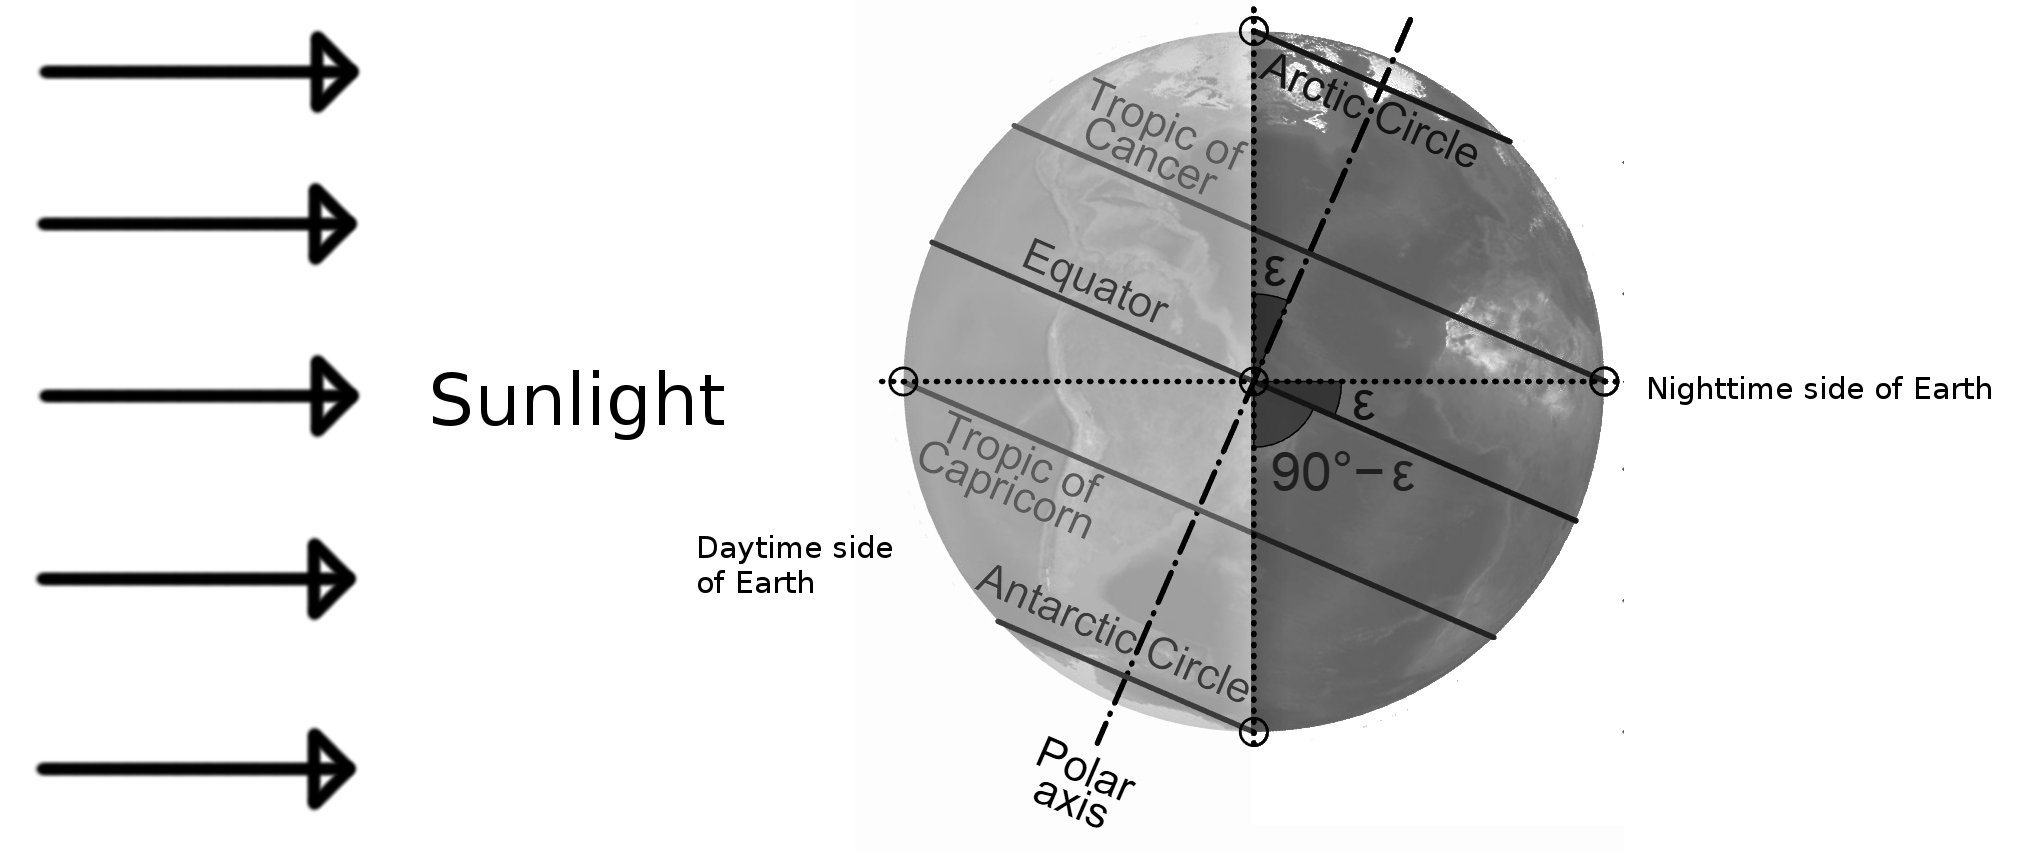
\includegraphics[width=4in]{earth-rotate-figure.jpg}
\end{center}

\vspace*{1.5cm}
\hrulefill\\

\textbf{Question 16.}

Based on what you've done so far, fill out the following table based on the above figure.
 You shouldn't need {\it Stellarium} to work these things out. For the position of the Sun
at noon, give both its altitude and its direction, for instance ``high in the northern sky'', ``on the southern horizon'', ``at the zenith'', etc.

\begin{center}
\begin{tabular}{|c| c |c|}
\hline
 & Hours of sunlight per day (approx.) & Position of Sun at noon \\
\hline
Arctic Circle & & \\
\hline
Antarctic Circle & &\\
\hline
Equator & & \\
\hline
Tropic of Cancer & 9 & \\
\hline
Tropic of Capricorn & & \\
\hline
\end{tabular}
\normalsize
\end{center}








\end{document}
